\section{Hall Thrusters}

\subsection{Working principles}

Hall Thrusters are a purely electric propulsion technology. As stated in \cite{fep_book}, they share the propulsive mechanism with ion thrusters: the propellant, usually Xenon, is ionized and accelerated through an electric field to provide thrust. However, the ionization process differs from a grid-based ion-thruster: the technology uses the eponym Hall-effect to capture a dense plasma of free electron through which the neutral propellant jet passes. This allows for a more compact and simpler design than ion thrusters, but often at the cost of efficiency and specific impulse.

\begin{figure}[H]
    \centering
    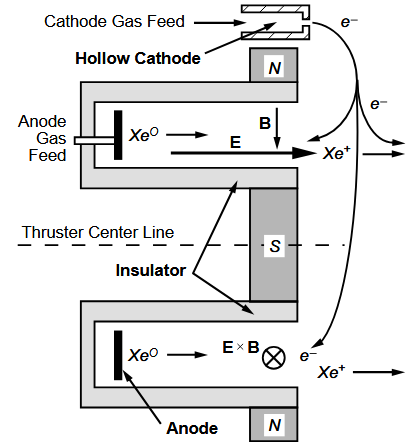
\includegraphics[width=0.3\linewidth]{figs/hall_thrusters_1.png}
    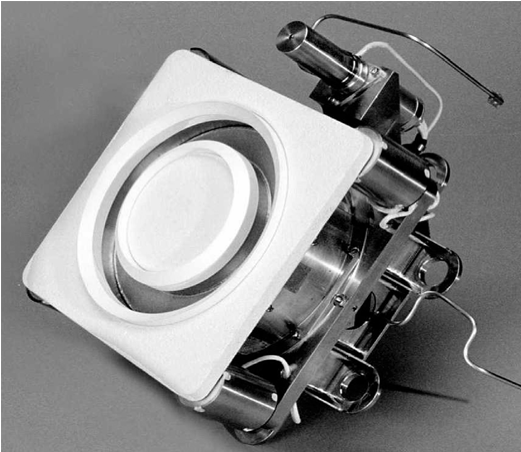
\includegraphics[width=0.3\linewidth]{figs/hall_thrusters_2.png}
    \caption{Left, a schematic of an Hall thruster. Right, an Hall thruster manufactured by Aerojet \cite{fep_book}}
    \label{het_illustration}
\end{figure}

The circular ring where the reaction takes place is called the channel. Magnets and an iron shunt are used to generate a strong radial magnetic field while an anode/cathode pair generates a longitudinal electric field. The cathode has two aditionnal roles: providing electrons for the plasma in the channel and jet neutralization.

The main advantage of this technology is that it isn't burdened by the charge limiting effect of standard ion thrusters and is therefore not space limited. Indeed, the propellant is  neutral throughout most the channel and is ionized only at the end of it, where the trapped electron plasma lies.

\subsection{The use of electromagnetic field}

As explained in \cite{demo_het}, the whole idea of an Hall thruster is to exploit the mass difference between electron ($9.109 \cdot 10^{-31}$kg) and ions (usually on the order of $10^{-26}$kg) so that the two particles have a different behaviour in the channel. Namely, ions are simply accelerated through the channel by the electric field and ejected to provide thrust while the electrons are captured by the magnetic field to generate the ionization plasma. Applying Newton first law to all of these particle, subjected to electromagnetic forces:

\begin{equation}
\label{eq:het_newton}
    m\vec{a} = q\vec{E} + q\vec{v}\times\vec{B}
\end{equation}

It follows that a charged particule tends to be accelerated along electric field lines and orbit magnetic field lines. The orbit radius, commonly refered as the Larmor radius, can be calculated as such, where $E_c$ is the kinetic energy of the particle:

\begin{equation}
\label{eq:het_larmor}
    r = \frac{\sqrt{2mE_c}}{qB}
\end{equation}

Considering only the effect of engine-generated electromagnetic field and not particle to particle interactions for simplification, it is posible calculate the two Larmor radius of electrons and ions. Since the radius depends on mass, the relation $r_e << r_i$ is generally verified. Hall thrusters are functional on the condition $r_e << l_c << r_i$, where $l_c$ is the length of the channel. Using cheap magnets whith peak field of 0.0270T, \cite{demo_het} found a Lamor radius of 0.33mm for electrons and 20m for ion, which allows for a comfortable dimensionning of the channel.

Under this condition, electrons are circling at the end of the channel and form a current (called Hall current), bombarding the passing ions, eventually ionizing some by collision. These ions are then ejected by the eletric field, providing thrust. Electrons will then either traverse the channel and close the circuit by contact with the anode or also be ejected.

\subsection{Efficiency}

The exhaust velocity of Hall Thrusters is simply $v_e = \sqrt{2eV_A/m_i}$, where $V_A$ is the acceleration voltage and $\dot{m_i}$ the mass flowrate of ions. The thrust efficiency is then, with $P$ the consumed electric power and $\dot{m_p}$ the mass flowrate of propellant:

\begin{equation}
\label{eq:het_threff}
    r = \frac{\sqrt{\dot{m_p}v_e^2}}{2P}
\end{equation}

Hall thrusters rely deeply on a efficient and quick ionization process in the channel. Denoting $N_a$ the density of neutral propellant in the plasma region of the channel, it appears that $N_a(z) = N_{a0}\exp(-z/L_i)$, where $L_i$ is the caracteristic length of ionization. Generally, this length shall be really small compared to the length of the channel. The length can be related to electron temperature $T_e$, electron density $n_e$ and speed of electron along the azimuth $u_{az}$, all of them derivable from operating parameters through plasma physics:

\begin{equation}
\label{eq:het_ionlen}
    T_e^{3/2} \sim \frac{L_i n_e}{u_{az}}
\end{equation}

The main power loss from an Hall Thruster comes from electrons in the Hall current colliding with the channel walls, eroding it and diminishing power of the Hall current. This power loss can be approximated trough, with $A_w$ the walls area:

\begin{equation}
\label{eq:het_wallloss}
    P_w \sim T_e^{3/2} n_e A_w
\end{equation}

%\subsection{Typical performances}

%This table is an extract from table 4.10 of \cite{nasa_report} and reports performances of the EDB Fakel SPT-50 Hall thruster (Russian thruster installed on Canopus-V). Refer to the source material for more example and details. As most of electric propulsion systems, Hall thrusters present a very high specific impulse (generally a bit higher than 1000s) but a poor thrust (in the order of a few cN).

%\begin{table}[H]
%\centering
%\caption {EDB Fakel SPT-50 Hall thruster performances}
%\label{tab:het_performance}
%\begin{tabular}{@{}ll@{}}
%\toprule
%\textbf{Parameter} & \textbf{Benchmark Value} \\ \midrule
%Thrust (mN) & 14 \\
%Specific Impulse (s) & 860 \\
%Total Impulse (kNs) & 126 \\
%Hardware Mass (kg) & 3.3 \\
%Propellant & Xenon \\\bottomrule
%\end{tabular}
%\end{table}